In this section, we use an alternate data source to validate the
findings in the body of the paper. We use the National Health
Interview Survey (NHIS), which is an annual repeated cross-section
survey of about 35,000 households and 87,000 individuals. Mortality
rates can be calculated directly from the NHIS, because NHIS records
are intermittently linked to death certificate records from the
National Death Index. We can therefore estimate a population subgroup
mortality rate as the share of individuals who are deceased in a given
followup period.

Because mortality rates and education/ethnicity are all measured for
the same individuals, there is no possibility of inconsistent measurement of ethnicity or education between death counts and population counts. For instance,
if some individuals without a high school education report that they
have a high school education, both their deaths and their population
will be counted among the high school group. This may create a small
bias if mortality is correlated with misreporting, but it will be
considerably less bias than if their deaths are counted in the dropout
group and their population is counted in the high school completion
group.  This said, NHIS-based measures of mortality slightly
underestimate aggregate mortality relative to vital statistics data,
especially for older white women, because the NHIS sample population appears to be more healthy than average \citep{ingram2008}.

We obtained public NHIS data with mortality followup for
NHIS participants linked to death records
through 2015. NHIS interviews occur
throughout the year.\footnote{The sample of deaths in the year following the NHIS
  survey is extremely small. In some of our subgroups, there were zero
  deaths reported in the shortest followup periods.} We aggregated
results across all ages using the standardized U.S. population
distribution, as in Section~\ref{sec:all_ages}. Because our aim in
this section is to validate the raw mortality estimates from the NCHS,
we present raw mortality change for education levels, rather than
bounding the mortality change in constant education percentiles.

Figure~\ref{fig:nhis_mort} below compares estimates of annualized
mortality change in the NHIS vs. our estimates from the NCHS for the
four key groups in our study: non-Hispanic white female dropouts and
high school completers, and non-Hispanic white male dropouts and high
school completers. Mortality change in the NHIS is calculated from
the average mortality in periods 1997--1999 to the last period in which the $n$-year mortality rate can be
calculated. For example, we can compute 1-year mortality for the 2014
data, 2-year mortality for the 2013 data, etc. 

The red points in Figure~\ref{fig:nhis_mort} show NHIS mortality estimates with 95\%
confidence intervals. Even with the 6-year followup period, the NHIS
sample is too small to precisely estimate mortality change over the
sample period. Most point estimates are very close to our mortality
change estimates from NCHS data (indicated by the dashed green line),
but in many cases the NHIS confidence interval includes both zero and
our measure. In almost all cases, our NCHS measure of mortality change
is within one standard error of the NHIS estimate and they are particularly close for the largest sample mortality followup in NHIS (6 years).\footnote{Compared with our
  results, NHIS calculates slightly higher mortality increases for high school completers and slightly lower for dropouts, but the opposite interpretation also falls within the confidence interval. The NHIS estimates are just not precise enough to make any clear statement about the difference between these groups.}

\textbf{Health status.} NHIS estimates of mortality are imprecise because the number of
middle-aged white dropouts in the sample who die is very small. We can
obtain more precise estimates of health status, which is reported by
all respondents. NHIS respondents are asked to report their perception
of their own health on a five point scale, where one reflects very
good health, and five reflects very bad health. In
Figure~\ref{fig:nhis_health}, we show the annualized change
in self-reported health status from 1997 to 2014 at each age and
education level, plotted with a lowess smoother.

The left panel shows the result for non-Hispanic white women. At most
ages, dropouts have experienced worse health declines than members of
any other group. Among 40--60-year-old women, self-reported health
status has gotten 0.0175 points worse \textit{per year}, or 0.2 points
worse on a 5 point scale from 1997 to 2009. The age pattern of the
health decline closely matches our mortality results in
Figure~\ref{fig:mort_main}, with the greatest divergence between
dropouts and high school graduates occurring between ages 40 and
60. We observe less change in the education-health gradient among men,
but dropouts suffer the worst relative deterioration in health between ages
50--70, corresponding exactly to the ages where we document the
greatest differential increases in mortality among the bottom 10\% in
Figure~\ref{fig:mort_main}.

In conclusion, measures of mortality and self-reported health in the
NHIS are broadly consistent with our findings of increased
mortality among middle-aged whites in the least educated
10\%. These NHIS measures are less precise than the vital statistics
mortality data, but they do not suffer from any division bias that
could be caused by changes in how individuals respond to questions
about their education or ethnicity over time.

\begin{figure}[H]
  \caption{Annualized Mortality Change Estimates from NHIS and from NCHS (1997--2015)}
  \label{fig:nhis_mort}
  \begin{center}
    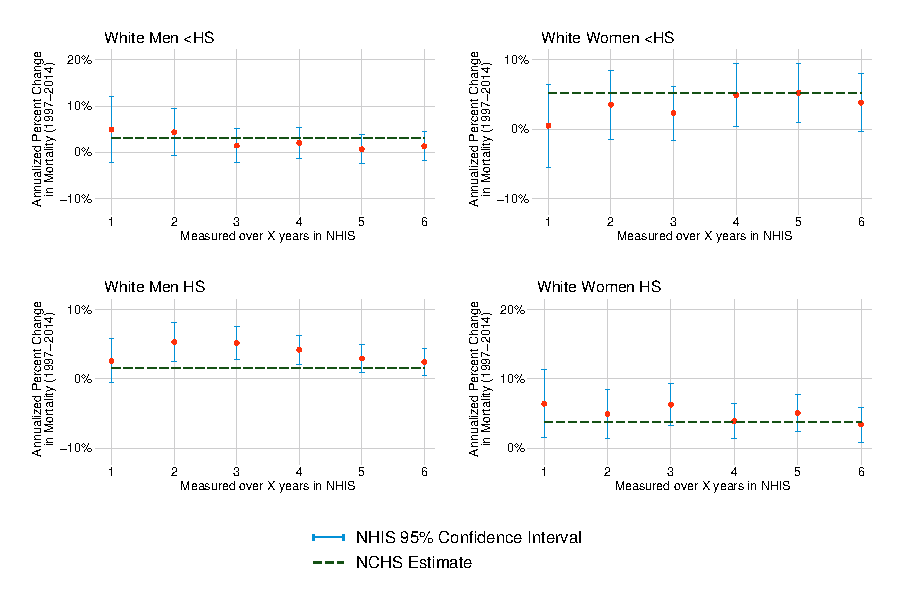
\includegraphics[scale=1.1]{\mortalitypath/ests_yline} \\
  \end{center}
\end{figure}
\scriptsize{The figure compares estimates of annualized mortality
  change in the National Health Interview Survey (NHIS) with vital
  statistics data from the NCHS, used in the body of the paper. The
  annualized change in the mortality rate from 1997--99 to 2015 according to
  NHCS (vital statistics data) is indicated by the dashed green
  line. The six different points for each panel reflect annualized
  mortality changes in the NHIS based on measurement of 1-year
  mortality, 2-year mortality, 3-year mortality, and so on. 1-year
  mortality is reported in the NHIS using 1997--1999 as a base period
  and comparing to participants interviewed in 2014 with mortality followup to 2015. 2-year
  mortality change is reported from 1997--1999 and comparing to 2013 participants,
  and so on. These different estimates are
  nevertheless comparable because the mortality change
  estimates are annualized. Standard errors are calculated for the
  NHIS using NHIS sample weights.}

\begin{figure}[H]
  \caption{Change in Self-Reported Health Status (NHIS, 1997--2015)}
  \label{fig:nhis_health}
  \begin{center}
    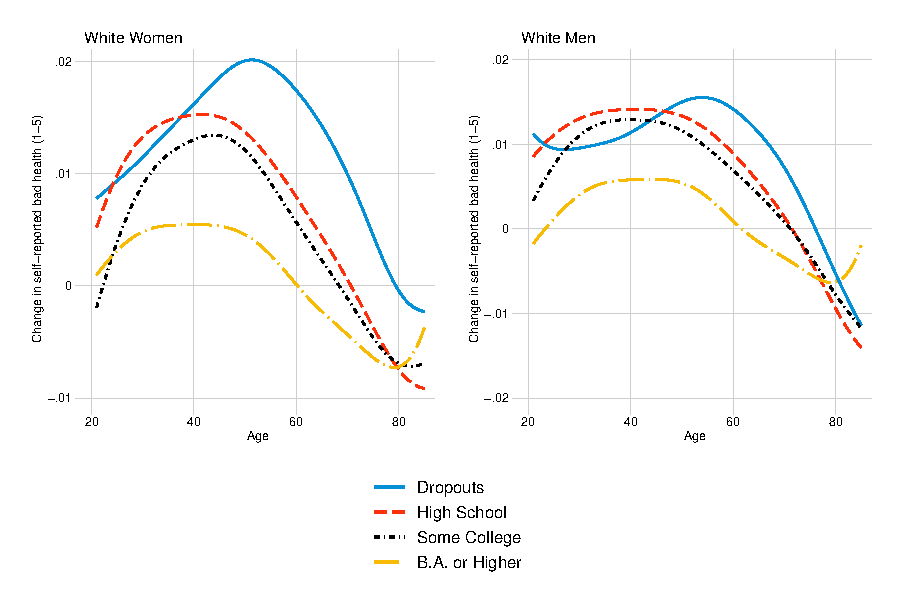
\includegraphics[scale=1.1]{\mortalitypath/lowess_sex_both} \\
  \end{center}
\end{figure}
\scriptsize{The figure shows a lowess fit to the annualized change in
  self-reported health from 1997 to 2015 at each age, according the
  NHIS. Self-reported health status is on a five point scale, where
  one represents the best health and five represents the worst.  We
  calculate annualized change for each age cohort / education group by
  regressing self-reported health status on a year variable. We then
  plot the year coefficients for each age/education group using a
  lowess smoother to minimize noise across single-year age
  cohorts. The series therefore shows the predicted change in
  self-reported health for an individual in a given age, gender and
  education group.}



